\chapter{Giới Thiệu Bài Toán}
\section{Lý do chọn đề tài}
Xe hơi tự lái từng là một câu chuyện viễn tưởng, thế nhưng công nghệ này đang dần được hoàn thiện và đang trong quá trình đưa vào thử nghiệm thực tiễn. Uber, Waymo, Tesla cùng hàng loạt những ông lớn công nghệ khác đã đổ hàng tỷ USD để nghiên cứu, phát triển một công nghệ hứa hẹn sẽ an toàn và hiệu quả hơn rất nhiều so với chính con người điều khiển ô tô. Không những vậy, Elon Musk \protect \footnotemark \footnotetext{Elon Musk là một nhà phát minh, doanh nhân, tỉ phú người Mỹ. Ông được biết đến với tư cách người sáng lập SpaceX, đồng sáng lập Tesla Motors và PayPal. Tại SpaceX ông là CEO và Trưởng bộ phận thiết kế và ở Tesla Motors ông là Chủ tịch, CEO và Kiến trúc sư sản phẩm} còn nói rằng Tesla có thể sản xuất ra ô tô tự lái hoàn toàn vào năm 2019.\par
Về cơ bản, xe tự lái sử dụng công nghệ giúp chúng có thể tự di chuyển, xác định phương hướng và nhận thức được môi trường xung quanh mà không cần đến con người tác động. Mỗi chiếc xe đều được trang bị một thiết bị GPS, hệ thống định vị nội bộ và các bộ cảm biến bao gồm máy định vị laser, radar và video.\par 

Khi đã có các trang bị hỗ trợ thì việc chúng phải tự nhận biết chướng ngại vật, phương tiện giao thông trên đường, người đi bộ, các biển báo,...có thể đang là vấn đề đầy thử thách. Trong đó việc phát hiện và phân loại biển báo trở nên phức tạp khi mà các yếu tố ngoại cảnh tác động. Biển báo có thể bị hư hại khi tiếp xúc một thời gian dài dưới ánh nắng mặt trời. Màu sắc bị thay đổi trong các điều kiện sương mù, ánh sáng yếu ban đêm, biển báo bị che khuất bởi nhà cửa, cây cối,... Vì thế khi biển báo được nhận dạng, phân loại một cách tự động và có thể nhận biết được các biển báo xuất hiện trên đường theo thời gian thực thì nó sẽ giúp ô tô có thể tự tuân thủ luật giao thông và tránh được các tai nạn nguy hiểm.\par
%Nguyên nhân của những vụ tai nạn giao thông trên chủ yếu do người điều khiển phương tiện đi sai phần đường, tránh vượt sai quy định, vi phạm tốc độ, chuyển hướng không quan sát hết biển báo giao thông.
%Chính vì thế, các nhà khoa học các nước tiên tiến trên thế giới nghiên cứu và đề xuất nhiều giải pháp như:
%\begin{itemize}
%\item[-] Nâng cao cơ sở hạ tầng giao thông tương ứng với tốc độ tăng trưởng kinh tế.
%\item[-] Tuyên truyền luật giao thông cho người tham gia giao thông đầy đủ để họ có thể nắm được và tham gia giao thông an toàn.
%\item[-] Giải pháp quan trọng nhất, nắm hoàn toàn sự thành công là giải pháp nâng cáo ý thức của người điều khiển phương tiện khi tham gia giao thông.
%\end{itemize}
Do đó khóa luận đã chọn đề tài là “Nghiên cứu về học sâu và ứng dụng cho bài toán nhận dạng biển báo giao thông”.
\begin{figure}[H]
\subfloat[Xe tự lái Google]
  {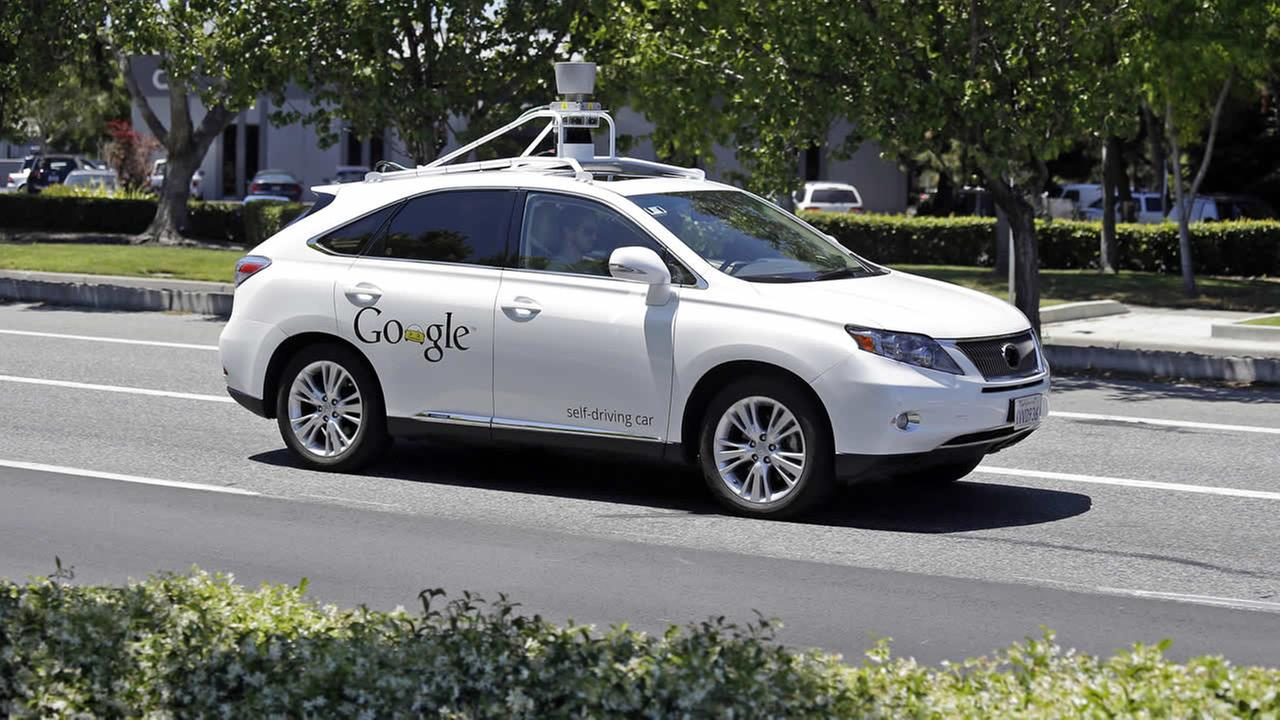
\includegraphics[width=.5\linewidth]{header/image/selfDriving.jpg}}\hspace{5mm}
\subfloat[Xe tự lái Tesla]
  {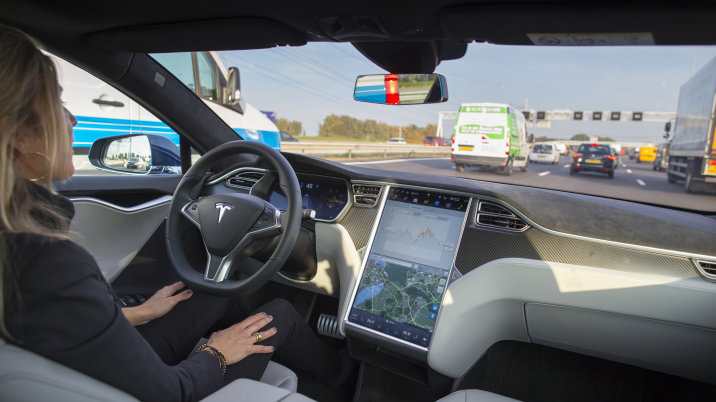
\includegraphics[width=.5\linewidth]{header/image/Tesla.jpg}}\hfill
\end{figure}
\section{Mục tiêu của đề tài}
Nghiên cứu, tìm hiểu về kiến trúc, cách hoạt động của mạng nơ-ron nhân tạo hay còn gọi là học sâu, cũng như một số thuật toán object detection (nhận dạng vật thể). Và một số vấn đề gặp phải khi xây dựng các mô hình cũng như phương pháp giải quyết.\par
Nghiên cứu, ứng dụng cho bài toán nhận dạng biển báo giao thông để có thể tích hợp vào hệ thống xe tự lái nói riêng cũng như phát triển cho bài nhận dạng, phân loại vật thể nói chung. 
\section{Một số nghiên cứu}
\subsection{Phương pháp dựa trên màu sắc}
Cách tiếp cận phổ biển với bài toán biển báo giao thông là dựa trên màu sắc \cite{trafficcolor} \cite{trafficcolor1}, tìm một vùng ảnh có chứa màu sắc đặc trưng, sử dụng phương pháp phân ngưỡng màu đơn giản hoặc phân ngưỡng ảnh cao cấp. Kết quả của vùng ảnh sau đó sẽ ngay lập được được xem như là biển báo giao thông hoặc thông qua giai đoạn tiếp theo xem như là vùng cần quan tâm.\par
Khuyết điểm chính của phương pháp này là trong thực tế màu sắc có xu hướng không đáng tin cập, mà phụ thuộc vào các thời điểm trong ngày, điều kiện thời tiết, bóng râm, cây cối che lấp,.... Không gian màu RGB được đánh giá là rất nhạy cảm với ánh sáng, do đó nhiều nhà nghiên cứu đã chọn phân ngưỡng màu sắc trong các không gian màu khác như HSI \cite{trafficcolor3}.
\begin{figure}[H]
\begin{center}
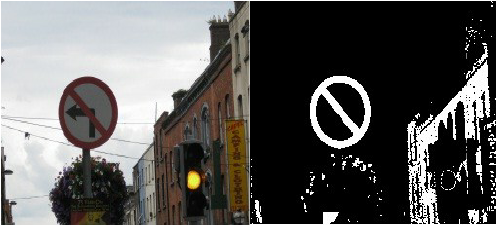
\includegraphics[scale=0.8]{header/image/detectbycolor.jpg}
\end{center}
\caption{Nhận diện dựa vào màu sắc}
\end{figure}
\subsection{Phương pháp dựa vào hình dạng}
Một khuyết điểm lớn trong phương pháp nhận dựa trên màu sắc đó là khi ánh sáng không tốt thì kết quả của chúng ta sẽ không được chính xác. Để khắc phục điều đó thì phương pháp dựa vào hình dạng vật thể đã được phát triển, đặc biệt là histogram of oriented gradients (HOG) \cite{dalal2005histograms}. Bản chất của phương pháp này là  phát hiện các thông tin về hình dáng và vẻ bề ngoài của các đối tượng cục bộ trong ảnh có thể được mô tả bằng cách sử dụng thông tin về sựphân bố của các cường độgradient (intensity gradients) hoặc của các hướng biên (edge directions). Sau đó dùng các thuật toán như support vector machine (SVM) \cite{mlcb}, K-nearest neighbors (KNN) \cite{mlcb} để phân loại ra các nhãn.
\begin{figure}[H]
\begin{center}
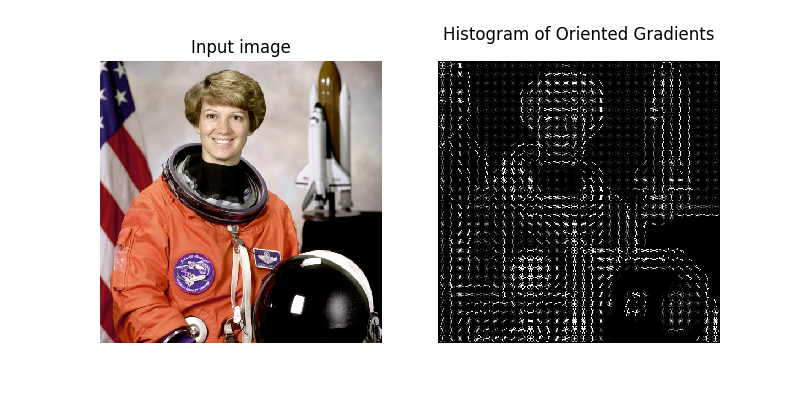
\includegraphics[scale=0.8]{header/image/hog_02.png}
\end{center}
\caption{Histogram of oriented gradients}
\end{figure}
